\documentclass[conference]{IEEEtran}
\IEEEoverridecommandlockouts
\usepackage[T1]{fontenc}
\usepackage{cite}
\usepackage{amsmath,amssymb}
\usepackage{graphicx}
\usepackage{booktabs}
\usepackage{url}
\usepackage{xcolor}
\usepackage{tikz}
\usetikzlibrary{positioning,arrows.meta,fit}

% DRAFT for the authors to rewrite. Every number comes from facts.json / the tab_*.tex files,
% which make_paper.py regenerates from the project results (python run_all.py).

\begin{document}
\bstctlcite{IEEEexample:BSTcontrol}

\title{CareGrid: Shielded Learning and Outage-Duration Forecasting to Protect Older Adults' Medical Devices During Heatwave Power Outages}

\author{\IEEEauthorblockN{Khrisha N$^{1,\dagger}$, Anushka Prasad$^{1,\dagger}$, Pushpa Mitra Ganesh$^{1,\dagger}$ and P. Madhavan$^{2,*}$}
\IEEEauthorblockA{$^{1}$\textit{Department of Electronics and Computer Engineering}\\
$^{2}$\textit{Department of Computing Technologies}\\
\textit{Faculty of Engineering and Technology, SRM Institute of Science and Technology}\\
Kattankulathur, Chennai, India\\
\{kn9023, ap0362, pg5197, madhavap\}@srmist.edu.in}
\thanks{$^{\dagger}$These authors contributed equally to this work. $^{*}$Corresponding author: P.~Madhavan (madhavap@srmist.edu.in).}}

\maketitle

\begin{abstract}
Older adults who depend on electrically powered medical equipment are among the people most at risk when a heatwave and a power outage coincide. Energy-management controllers usually express medical priority as a weight, which trades it against comfort and leaves safety to tuning. CareGrid enforces medical service at run time instead. A shield serves devices in three priority tiers, holds a battery reserve sized to a worst-case restoration time, refills it from solar, and spends the remaining energy on cooling ordered by a rule-based health twin of resident heat vulnerability. Learned policies act only inside the shield: PPO-Lagrangian for a community battery and multi-agent PPO-Lagrangian (MAPPO) for homes with their own batteries. A quantile model trained on 6,053 Arizona outages from the EAGLE-I record supplies the worst-case restoration time. In a Phoenix microgrid simulation driven by July 2023 weather, the shield cut unpowered medical device-hours per outage from 103.8 under weighted priority to 0.1, and stayed at or below 0.9 on 48\,h outages under solar-forecast error, sensor bias and smaller batteries. Ordering cooling by the health twin lowered vulnerability-weighted heat exposure by 11.1\%. After a 24\,h warning, PPO-Lagrangian lowered it by a further 2.4\% relative to fixed pacing; without a warning the reserve left it no choice to make. On CityLearn v3 homes in Austin, the shield cut losses from 81.4 to 6.1 device-hours, and on unseen test outages MAPPO lowered them from 3.4 under fixed pacing to 1.3, at the price of 4.8\% more weighted heat exposure. The forecaster's 90th percentile covered 89\% of unseen 2023--24 outages.
\end{abstract}

\begin{IEEEkeywords}
Energy resilience, power outages, older adults, safe reinforcement learning, shielding, multi-agent reinforcement learning, outage duration, microgrids, health digital twin
\end{IEEEkeywords}

\section{Introduction}
Heatwaves and power outages increasingly arrive together, and the combination is far more dangerous than either alone. Across U.S.\ counties from 2015 to 2019, each hour of outage on a hot day increased the mortality harm of that day by 61\%, with the elderly among the groups most affected \cite{ai2025heat}. Modelling of historical heatwaves suggests that a multiday blackout during a heatwave would more than double heat-related mortality and would require medical attention for more than half of Phoenix's population \cite{stone2023blackouts}. Outages are also associated with cardiovascular and respiratory hospitalizations among Medicare beneficiaries \cite{mcbrien2026outages}. More than 4.5 million U.S.\ Medicare beneficiaries living independently rely on electricity-dependent medical equipment or services \cite{empower}, and rentals of such equipment more than doubled across most demographic groups between 2008 and 2018 \cite{casey2021dme}. Outage vulnerability is unevenly distributed \cite{dugan2025survey,ezzati2025porsvi}, and older people face distinct risks in the energy transition \cite{zuk2024ageism}.

Rooftop solar, batteries and community microgrids can bridge outages, but they do not remove the allocation problem: when an islanded system runs short, something has to be switched off, and the restoration time is unknown. Energy-management systems for older adults optimise comfort and cost while the grid is up \cite{athanasiadis2022sems,tsaknakis2023nearly,kaculi2025human}. Resilience-oriented controllers, including multi-agent reinforcement learning (MARL), maximise generic critical-load service or minimise cost \cite{wu2026marl,qiu2023repair,esan2026lean}. Gong \textit{et al.}\ showed that adding the settlement cost of durable-medical-equipment (DME) users to an offline load-shedding optimisation cut DME exposure by 77.6\% \cite{gong2026dilemma}. Across this work, vulnerability enters as a weight or cost term.

A weight is the wrong instrument for a life-safety requirement. Its effect depends on tuning, it is traded continuously against comfort, and it does not account for the uncertain length of the outage, which decides whether energy spent now is energy missing later. Safe reinforcement learning offers an alternative: constrained policy optimisation \cite{achiam2017cpo,stooke2020pid,ray2019safety} and runtime shields that override unsafe actions \cite{alshiekh2018shield}. A shield, however, needs a worst-case restoration time, and a learned policy inside it needs room to act. This paper studies both.

Our contributions are:
\begin{enumerate}
\item A policy-agnostic runtime shield for islanded communities of older adults. It serves medical devices in three priority tiers, holds a battery reserve to a worst-case restoration time, refills that reserve from solar, and allocates thermal-safety cooling by a rule-based health twin of resident heat vulnerability.
\item Learning inside the shield with two methods: a PPO-Lagrangian policy that paces a community battery, and a MAPPO-Lagrangian policy with one agent per home and centralised critics. Both are evaluated on held-out outages over several seeds, with shield, health-twin and warning ablations.
\item A restoration-time forecaster trained on ten years of public county-level outage records (EAGLE-I \cite{brelsford2024eaglei}), with calibrated 90th-percentile estimates, and a test of what happens when its estimates drive the shield.
\item An evaluation on two platforms driven by measured weather and building data, our Phoenix simulator and CityLearn v3, against the status quo, rule-based, weighted greedy and model-predictive controllers and performance bounds. It includes robustness to solar-forecast error, sensor bias and battery size over 28 start days and a measurement of the heat-exposure price of the medical guarantee.
\end{enumerate}

\section{Related Work}
\textit{Energy management for older adults.} Athanasiadis \textit{et al.}\ \cite{athanasiadis2022sems} and Tsaknakis \textit{et al.}\ \cite{tsaknakis2023nearly} control thermal, storage and appliance loads in elderly households, using load disaggregation to monitor activity. Kaculi \textit{et al.}\ \cite{kaculi2025human} design demand response around the comfort of ageing occupants. Digital twins of older adults are emerging \cite{lehmann2024twins,momand2025twins}, but they are not yet coupled to energy dispatch. These systems assume a grid connection and treat comfort as an objective.

\textit{Microgrid resilience and learning.} MARL has been used to keep microgrids running through typhoons \cite{wu2026marl}, to dispatch repair crews \cite{qiu2023repair} and to manage networked microgrids under uncertainty \cite{esan2026lean}. Cognitive and edge-coordinated digital twins approach optimal microgrid operation in practice \cite{sivaneasan2025cognitive,vanitha2025cet}. MAPPO, which shares an actor between agents and trains centralised critics, is a strong baseline for cooperative MARL \cite{yu2022mappo}. None of these treats a person's medical equipment as a constraint.

\textit{Equity in load shedding.} Gong \textit{et al.}\ \cite{gong2026dilemma} is the closest work. They optimise a single offline curtailment decision with a DME-aware cost. We address online, hour-by-hour control of islanded resources under an uncertain restoration time, enforce medical service as a constraint rather than a cost, and let learned policies act only inside that constraint.

\textit{Outage records.} EAGLE-I records the number of customers without power in every U.S.\ county at 15-minute intervals since 2014 \cite{brelsford2024eaglei}. We use it to learn conditional quantiles of outage duration \cite{koenker1978quantile} with gradient boosting \cite{friedman2001gbm}, so that the shield's worst-case time comes from data rather than from an assumption.

\section{Problem Formulation}
\subsection{Islanded system}
A set of buildings $\mathcal{H}$ is islanded from hour $t_0$ until an unknown restoration time $\tau$. Building $h$ has residents $\mathcal{N}_h$ and medical devices $\mathcal{D}_h$. Each device draws $p_d(t)$ on its schedule and belongs to a priority tier $\pi_d\in\{1,2,3\}$: P1 life-sustaining (oxygen concentrators, ventilator), P2 medical storage (insulin and medication fridges), P3 other health equipment (CPAP, wheelchair charger). Each hour the controller chooses device states $x_{d,t}\in\{0,1\}$, essential-circuit power $e_{h,t}$ and cooling power $u_{h,t}$, subject to
\begin{gather}
\textstyle\sum_{h}\big(\sum_{d\in\mathcal{D}_h} x_{d,t}\,p_d(t) + e_{h,t} + u_{h,t}\big) + c_t = P_t + d_t - s_t, \\
E_{t+1} = E_t + \eta c_t - d_t/\eta, \\
E_{\min}\le E_t\le E_{\max},\qquad 0\le c_t,d_t\le \bar P,
\end{gather}
where $P_t$ is solar output, $E_t$ battery energy, $c_t,d_t$ charge and discharge, and $s_t\ge 0$ curtailment. Indoor temperature follows a grey-box model
\begin{equation}
T_{h,t+1} = T_{h,t} + \tfrac{1}{C_h}\!\left[\tfrac{T^{o}_t - T_{h,t}}{R_h} + a_h G_t + q_h - \mathrm{COP}(T^{o}_t)\,u_{h,t}\right]
\end{equation}
(in CityLearn, the platform's per-home LSTM replaces it).

\subsection{Health twin}
Each resident $n$ receives a heat-vulnerability weight $v_n = 1 + a_n + \sum_{k} c_{n,k}$, where $a_n$ is 0.25 for ages 75--84 and 0.5 from 85, and $c_{n,k}$ adds 0.4 for respiratory or cardiovascular disease, 0.3 for cognitive impairment, 0.25 for diabetes, 0.2 for reduced mobility and 0.1 for sleep apnoea. These follow the factors that impair thermoregulation or heat avoidance in older adults \cite{kenny2010heat}. Building $h$ carries $V_h=\sum_{n\in\mathcal{N}_h} v_n$. The increments are illustrative design values, not a validated clinical score.

\subsection{Objectives under restoration uncertainty}
We define unserved critical energy $J_1=\sum_t\sum_d p_d(t)(1-x_{d,t})$, vulnerability-weighted heat exposure $J_2=\sum_t\sum_h V_h\,[T_{h,t}-T_c]^+$ with $T_c=26.7^\circ$C, and unserved essential energy $J_3$. The intended preference is lexicographic: $J_1$, then $J_2$, then $J_3$. The controller knows the utility's point estimate $\hat\tau$ and a conservative bound $\tau_{90}$, but not $\tau$. A weighted controller minimises $w_c J_1 + w_h J_2 + w_e J_3$. A constrained controller minimises $J_2$ and $J_3$ subject to $J_1=0$ whenever that is feasible.

\section{Method}
\subsection{The CareGrid shield}
The shield sits between any policy and the plant (Fig.~\ref{fig:shield}). Every hour it:
\begin{enumerate}
\item serves medical devices from the available supply $S_t = P_t + \min(\bar P, \eta(E_t - E_{\min}))$ in tier order P1, P2, P3;
\item computes a reserve that carries all devices to the worst-case restoration time, net of a conservative persistence forecast of solar output,
\begin{equation}
R_t = \sum_{k=1}^{H_t}\Big[\textstyle\sum_{d} p_d(t+k) - \alpha P_{t+k-24}\Big]^+,
\end{equation}
where $H_t=\max(H_{\min},\,\tau_{90}-t)$, $\alpha=0.7$ and $H_{\min}=12$\,h;
\item when stored energy is below $R_t$, routes surplus solar to the battery, up to its power limit and net of round-trip losses, before any non-critical use;
\item releases a non-critical budget from energy above the reserve,
\begin{equation}
\begin{aligned}B_t=\min\!\Big\{&S_t-\kappa_t,\\ &\tilde P_t+\min\!\big(\bar P-b_t,\;\rho_t\,[E^{a}_t-b_t-R_t]^+\big)\Big\},\end{aligned}
\end{equation}
where $\kappa_t$ is the critical power served, $b_t$ the part drawn from the battery, $E^{a}_t$ the deliverable stored energy, $\tilde P_t$ the solar left after critical loads and refilling, and $\rho_t$ the release fraction: $1/\max(1,\hat\tau-t)$ for the fixed-pacing shield, chosen by the policy otherwise;
\item spends $B_t$ first on thermal-safety cooling that holds each home at $T_c$ for the next hour, highest $V_h[\tilde T_h-T_c]^+$ first, where $\tilde T_h$ is the indoor temperature expected without cooling, and then on the policy's proposal for extra cooling, essential and discretionary loads.
\end{enumerate}
The shield never ranks one resident's medical devices against another's comfort. It guarantees each device a service floor and leaves comfort to the policy it wraps.

\begin{figure}[t]
\centering
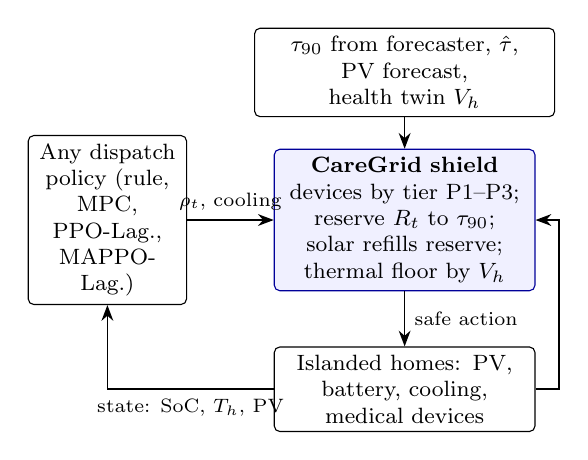
\begin{tikzpicture}[font=\footnotesize,
  box/.style={draw, rounded corners=2pt, align=center, inner sep=3pt, minimum height=8mm},
  arr/.style={-{Stealth[length=2mm]}, semithick}]
\node[box, text width=18mm] (pol) {Any dispatch\\policy (rule,\\MPC, PPO-Lag.,\\MAPPO-Lag.)};
\node[box, right=11mm of pol, text width=31mm, fill=blue!6, draw=blue!60!black] (sh) {\textbf{CareGrid shield}\\devices by tier P1--P3;\\reserve $R_t$ to $\tau_{90}$;\\solar refills reserve;\\thermal floor by $V_h$};
\node[box, above=4mm of sh, text width=36mm, minimum height=6mm] (fc) {$\tau_{90}$ from forecaster, $\hat\tau$,\\PV forecast, health twin $V_h$};
\node[box, below=7mm of sh, text width=31mm] (pl) {Islanded homes: PV,\\battery, cooling,\\medical devices};
\draw[arr] (pol) -- node[above, font=\scriptsize]{$\rho_t$, cooling} (sh);
\draw[arr] (fc) -- (sh);
\draw[arr] (sh) -- node[right, font=\scriptsize]{safe action} (pl);
\draw[arr] (pl.west) -| node[pos=0.25, below, font=\scriptsize]{state: SoC, $T_h$, PV} (pol.south);
\draw[arr] (pl.east) -- ++(3mm,0) |- (sh.east);
\end{tikzpicture}
\caption{The CareGrid shield wraps any dispatch policy. The policy proposes how much energy above the reserve to release and where to send extra cooling; the shield enforces medical service, a worst-case reserve and a vulnerability-ordered thermal floor before passing the action to the islanded system.}
\label{fig:shield}
\end{figure}

\subsection{Learning inside the shield}
The learned policies choose only what the shield leaves open: the release fraction $\rho_t$ and, for the community, how extra cooling is shared. Medical service is never an action. Both are trained with a Lagrangian relaxation \cite{ray2019safety}: the reward is $r_t=-\sum_h V_h[T_{h,t+1}-T_c]^+/20$, the cost $c_t$ is person-hours above $32.2^\circ$C, and after each batch the multiplier is updated as $\lambda\leftarrow\max(0,\lambda+0.05(\bar c-d))$, with $d$ set to 80\% of the cost rate of the fixed-pacing shield (for MAPPO, of its initial policy, which starts near fixed pacing). Neither policy observes the true duration $\tau$.

\emph{PPO-Lagrangian (community battery).} One agent controls the Phoenix community battery. Its action $a_t\in[-1,1]^{10}$ gives $\rho_t=((a_{t,0}+1)/2)^2$ and cooling shares $\mathrm{softmax}(2a_{t,1:9})$ for the nine buildings. Its 29-dimensional observation holds battery state, elapsed time, time of day, current and 3\,h persistence-forecast solar, current and 3\,h-ahead outdoor temperature, reserve, free energy above the reserve, time left to $\hat\tau$, and each building's sensed indoor temperature and vulnerability-weighted risk. We use PPO \cite{schulman2017ppo} from Stable-Baselines3 \cite{raffin2021sb3} with two 64-unit layers, 2,048 steps per update, minibatch 256, learning rate $3\times10^{-4}$, $\gamma=0.99$ and GAE $0.95$, for 200,704 steps, and train the policy on $r_t-\lambda c_t/20$.

\emph{MAPPO-Lagrangian (one agent per home).} In CityLearn each of the ten homes has its own battery and is one agent. All agents share one actor that sees only its home's 14-dimensional observation (battery, time, solar, weather, indoor temperature, reserve, free energy, time left to $\hat\tau$, $V_h$, device load and cooling need) and outputs $\rho_{h,t}=\sigma(x)$, $x\sim\mathcal{N}(\mu_\theta,\sigma^2)$. Separate reward and cost critics see the concatenated 140-dimensional state during training only \cite{yu2022mappo}. The policy update uses the clipped ratio (0.2) of the joint action with the combined advantage $(A^r-\lambda A^c)/(1+\lambda)$, eight epochs, Adam at $3\times10^{-4}$, and eight outages per update for 320 outages per seed. The actor's output bias is initialised near the fixed-pacing release.

\subsection{Restoration-time forecaster}
From EAGLE-I \cite{brelsford2024eaglei} we take all Arizona county records for 2015--2024. An event starts when at least 100 customers in a county are out, continues while they stay out with gaps of at most 30 minutes, and counts only if at least 1,000 customers are out at its peak. This gives 6,053 events. The target is log duration. The features are month, hour, weekday, summer, the number of customers out in the first hour and the county's customer count (both $\log_{10}$), all known within an hour of onset. We fit gradient-boosted quantile regression \cite{friedman2001gbm,koenker1978quantile} for the 50th and 90th percentiles (scikit-learn \cite{pedregosa2011sklearn}; 300 trees of depth 3, learning rate 0.05, at least 20 samples per leaf) on 2015--2021 (3,579 events), set 2022 aside, and test on 2023--2024 (1,643 events). The baseline is the training-set quantile. For the simulated scenario, a weekday outage in Maricopa County starting at 14:00 in July, the model gives $\tau_{90}$ for a typical and a large event (the median and 90th percentile of first-hour size among 229 past summer-afternoon Maricopa events).

\section{Experimental Setup}
\subsection{Baselines}
\emph{Equal curtailment}, the status quo, scales all loads by the same fraction; a device receiving less than full power trips. \emph{Rule-based} control serves devices, then essential circuits, and cools only while the battery is above 40\% or from instantaneous solar. \emph{Weighted greedy} control ranks loads by value per kWh: $w_c=10$ for devices, 2 for essential circuits, and a heat weight $w_h$ times resident-scaled heat risk for cooling, paced to $\hat\tau$. \emph{Weighted MPC} solves a receding-horizon linear program (HiGHS \cite{huangfu2018highs}) to $\hat\tau$ (at least 12\,h) with perfect weather and solar forecasts; we also test a critical weight of 1,000 and a horizon of $\tau_{90}$. \emph{Shielded} variants wrap the greedy, MPC and learned policies; \emph{fixed pacing} is the shield with $\rho_t=1/\max(1,\hat\tau-t)$. Bounds are a \emph{perfect-foresight} linear program that knows $\tau$ and relaxes device states to $[0,1]$, and, in CityLearn, \emph{medical-only} dispatch.

\subsection{Platform 1: Phoenix community microgrid}
Eight households and a six-resident care facility (17 residents, $\sum_h V_h=27.4$) share 12 medical devices: five 350\,W oxygen concentrators and a 150\,W ventilator (P1), three 120--150\,W medication fridges (P2), and two 60\,W night-time CPAP machines and a 300\,W wheelchair charger (P3). They share 60\,kWp of PV and a 150\,kWh, 60\,kW battery ($\eta=0.95$). Hourly temperature and irradiance for 30 June to 3 August 2023, peaking at 46.8$^\circ$C, come from ERA5 \cite{hersbach2020era5} via Open-Meteo \cite{zippenfenig2023openmeteo}; the non-cooling load shape comes from NREL ResStock for Maricopa County \cite{wilson2022eulp}. The thermal model ($R_h=1.75^\circ$C/kW, $C_h=6$\,kWh/$^\circ$C per home-equivalent) uses 55.9\,kWh/day of cooling in July 2023, against 51.1\,kWh/day in ResStock for the cooler July 2018. While grid-connected, the battery runs self-consumption with a 30\% backup reserve. A JavaScript port used for an interactive demonstrator matches the Python simulator to within $3.6\times10^{-12}$ on 128 scenarios.

\subsection{Platform 2: CityLearn v3}
We use CityLearn 3.0.2 \cite{fonseca2026citylearnv3,nweye2025citylearn} with its \texttt{tx\_travis\_county\_neighborhood} dataset: ResStock homes in Austin, TX, with per-home LSTM thermal models and measured 2018 weather. Ten homes with summer cooling host similar households (14 residents, 12 devices), each with 6\,kW of PV from PVWatts v8 \cite{dobos2014pvwatts} and a 13.5\,kWh, 5\,kW battery. During outages each home runs a critical-loads panel (0.35\,kW of essential circuits plus its devices, water heater off). In CityLearn 3.0.2's built-in outage mode, batteries cannot discharge, because discharge is capped by a local-load estimate computed before loads are energised and net of solar. We therefore run CityLearn grid-connected, serve outage-hour loads only from PV and battery in the controller layer, and count any grid import CityLearn records as unserved energy, charged to medical devices first. This platform uses the base shield, without tiers or the health-twin floor.

\subsection{Scenarios and metrics}
Outages begin at 14:00 on each of 1--28 July with true durations of 12, 24, 48 and 72\,h (112 outages). Every controller is told $\hat\tau=24$\,h; unless stated otherwise the shield uses $\tau_{90}=48$\,h. Each scenario is run with and without a 24\,h warning, which pre-charges the battery from 30\% to full at a cost of 111\,kWh of grid energy in Phoenix. Learned policies train on outages starting 1--20 July and are tested on the 32 unseen outages starting 21--28 July, over five seeds (Phoenix) or three (CityLearn). Sweeps vary the heat weight $w_h\in\{0.25,\dots,8\}$, battery size, $\tau_{90}$, start hour, the PV forecast factor $\alpha\in\{0.4,0.7,1.0\}$ and a temperature-sensor bias of $\pm2^\circ$C. The primary metric is unpowered medical device-hours. We also report critical energy served, person-hours indoors above $32.2^\circ$C (PH$_{32}$, the U.S.\ National Weather Service ``extreme caution'' level), person-degree-hours (PDH) and vulnerability-weighted degree-hours (VDH, $J_2$) above $26.7^\circ$C. Paired comparisons use Wilcoxon signed-rank tests and 95\% bootstrap intervals (10,000 resamples of outages); learned policies are averaged over seeds per outage before pairing.

\begin{table*}[t]
\centering
\caption{Outage results without warning, mean over 28 start days $\times$ 4 durations ($n=112$). Device-h: medical device-hours unpowered per outage. Crit.: critical energy served. PH$_{32}$: person-hours indoors above 32.2$^\circ$C. PDH: person-degree-hours above 26.7$^\circ$C. Phoenix uses the full shield (priority tiers, reserve refill, health-twin thermal floor); CityLearn uses the base shield. --: not run on that platform.}
\label{tab:main}
\begin{tabular}{lrrrrrrr}
\toprule
 & \multicolumn{4}{c}{Phoenix community microgrid} & \multicolumn{3}{c}{CityLearn v3, Austin} \\
\cmidrule(lr){2-5}\cmidrule(lr){6-8}
Controller & Device-h & Crit.\ (\%) & PH$_{32}$ & PDH & Device-h & Crit.\ (\%) & PH$_{32}$ \\
\midrule
Equal curtailment (status quo) & 374.0 & 4.2 & 450 & 4{,}164 & 209.2 & 40.0 & 12 \\
Rule-based critical-first & 148.6 & 67.9 & 511 & 4{,}799 & 104.8 & 71.2 & 30 \\
Priority as weight, greedy & 103.8 & 82.0 & 409 & 4{,}073 & 81.4 & 81.4 & 32 \\
Priority as weight, MPC & 0.8 & 99.9 & 345 & 3{,}727 & -- & -- & -- \\
\quad MPC, critical weight $\times$100 & 0.8 & 99.9 & 345 & 3{,}727 & -- & -- & -- \\
\quad MPC planned to P90 & 0.3 & 100.0 & 336 & 3{,}723 & -- & -- & -- \\
\textbf{CareGrid shield} & 0.1 & 100.0 & 425 & 4{,}211 & 6.1 & 98.3 & 44 \\
Medical-only dispatch (bound) & -- & -- & -- & -- & 2.2 & 99.0 & 340 \\
Perfect-foresight optimum (bound) & 0.0 & 100.0 & 320 & 3{,}613 & -- & -- & -- \\
\bottomrule
\end{tabular}
\end{table*}


\section{Results}
\subsection{Medical service}
Table~\ref{tab:main} summarises the full grid. With weighted priority, the greedy controller left medical devices unpowered for 103.8 device-hours per outage in Phoenix and 81.4 in CityLearn. Inside the shield the same controller lost 0.1 and 6.1 ($p=1.6\times10^{-15}$ and $8.5\times10^{-19}$), while equal curtailment lost 374 and 209. Fig.~\ref{fig:duration} shows that weighted priority degrades with outage length. Fig.~\ref{fig:case} shows why. On the hottest afternoon the weighted controller runs the battery down to its floor within 14 hours and drops up to all 12 devices that night and the next, while the shield refills its reserve from the afternoon sun and keeps every device powered. The care facility's indoor temperature is almost the same under both. In CityLearn the base shield stays within 3.6 device-hours of the medical-only bound up to 48\,h. At 72\,h, beyond $\tau_{90}$, it loses 14.9 against 2.9.

\begin{figure}[t]
\centering
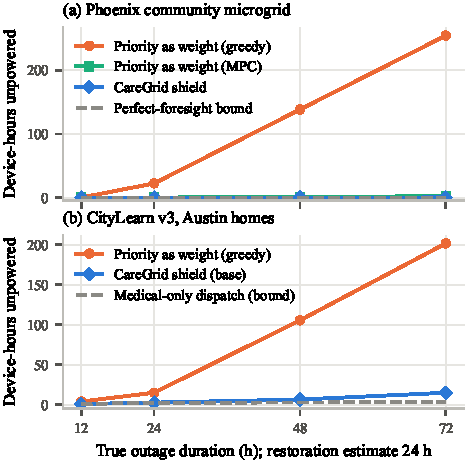
\includegraphics[width=\columnwidth]{fig_duration.pdf}
\caption{Unpowered medical device-hours against true outage duration (mean of 28 start days, no warning). Every controller assumes a 24\,h outage.}
\label{fig:duration}
\end{figure}

\begin{figure*}[t]
\centering
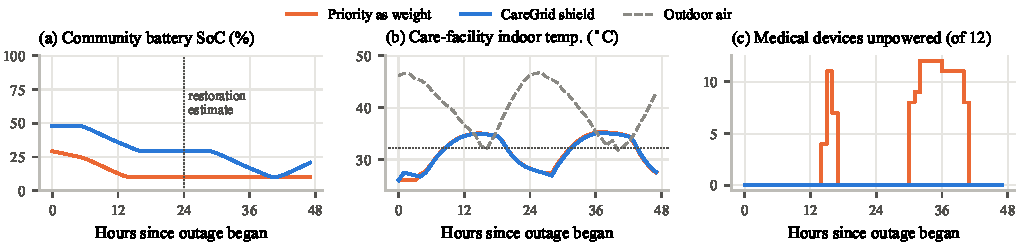
\includegraphics[width=\textwidth]{fig_case.pdf}
\caption{Phoenix case study: 48\,h outage from 14:00 on 19 July 2023, no warning. The weighted controller exhausts the battery on the first evening and leaves up to all 12 medical devices unpowered; the shield refills its reserve from solar and keeps every device powered, at almost no cost in care-facility temperature.}
\label{fig:case}
\end{figure*}

\subsection{Sensitivity of weighted priority}
A weighted MPC with perfect weather and solar forecasts was nearly safe at its default weights (0.8 device-hours per outage), but its safety depended on the weights. On 48\,h outages it lost 0.0--0.8 device-hours for $w_h\le1$, 386 for $w_h=2$ and 472 for $w_h\ge4$; the weighted greedy controller rose from 138 to 406. Starting the outage at 20:00 instead of 14:00 raised the MPC's losses from 0.8 to 39.1. The shield lost 0.1 or fewer at every weight, start hour, battery size from 75 to 400\,kWh and $\tau_{90}$ from 24 to 96\,h. An MPC planned to $\tau_{90}$ with perfect forecasts was also safe in these sweeps (0.3 device-hours pooled), so a carefully configured optimiser can protect devices; the shield does so without perfect forecasts and for any policy it wraps. In CityLearn the weighted greedy controller lost 104--106 device-hours at every heat weight: its failures came from spending stored energy early, which no weight corrected.

\subsection{Health twin}
Ordering the shield's thermal floor by vulnerability-weighted risk instead of building order cut VDH by 11.1\% (7,413 to 6,591), better on all 112 Phoenix outages ($p=4\times10^{-20}$). PDH fell by 6.1\% and PH$_{32}$ from 428.9 to 425.0 ($p=0.04$), with medical service unchanged (Table~\ref{tab:ablations}).

\subsection{Restoration-time forecaster}
Recorded outages are much shorter than the multi-day events the simulations test (Fig.~\ref{fig:forecast}a). The median Arizona event lasted 2.0\,h and the 90th percentile 9.3\,h; 7.0\% lasted at least 12\,h and 0.4\% (24 events) at least 48\,h, with a maximum of 262\,h. On the unseen 2023--24 events the forecaster's 90th percentile covered 89\% of outages (target 90\%) and its median 48\% (target 50\%), and its pinball loss was 10.8\% and 12.4\% lower than the training-set quantiles. Coverage held across the range of predicted values (Fig.~\ref{fig:forecast}b). The historical 90th percentile covered 94\% and is therefore more conservative than needed. For the simulated July afternoon in Maricopa County the forecaster gave $\tau_{90}$ of 5.7\,h for a typical and 7.4\,h for a large event, with medians of 1.8 and 2.2\,h.

Both forecasts fall below the shield's 12\,h minimum horizon, so in the shield they amount to a 12\,h reserve instead of 48\,h. With a warning this lowered VDH by 1.6\% (5,677 to 5,589, $p=1\times10^{-19}$) with medical service unchanged. Without a warning the battery starts below either reserve, and the change was 0.3\% (95\% interval $-47$ to $+7$). Also using the forecast median as the restoration estimate $\hat\tau$ made fixed pacing release the battery over about two hours. Against simulated outages of 12--72\,h this raised VDH by 4.9\% with a warning ($p=1\times10^{-8}$). The forecast median is a poor pacing target when the outage may be a heatwave-scale event far beyond the historical record.

\begin{figure}[t]
\centering
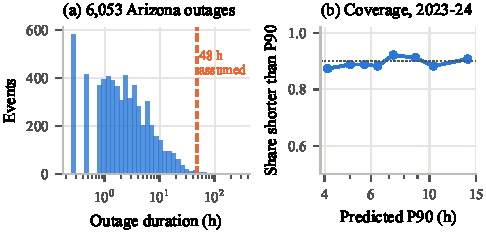
\includegraphics[width=\columnwidth]{fig_forecast.pdf}
\caption{(a) Durations of 6,053 Arizona outages in EAGLE-I, 2015--2024; the simulated shield assumes $\tau_{90}=48$\,h. (b) Share of unseen 2023--24 outages shorter than the predicted 90th percentile, in eight equal-size bins of the prediction.}
\label{fig:forecast}
\end{figure}

\begin{table}[t]
\centering
\caption{Learning inside the shield on unseen test outages (starts 21--28 July, 12--72\,h, $n=32$). Learned policies: mean $\pm$ s.d.\ over seeds (5 Phoenix, 3 CityLearn). VDH: vulnerability-weighted degree-hours above 26.7$^\circ$C. The perfect-foresight bound minimises unweighted heat exposure, so it bounds medical service and PH$_{32}$-related heat but not VDH.}
\label{tab:learning}
\setlength{\tabcolsep}{2.5pt}
\begin{tabular}{lrrr}
\toprule
Controller & Device-h & PH$_{32}$ & VDH \\
\midrule
\multicolumn{4}{l}{\textit{Phoenix, no warning}} \\
Priority as weight & 105.0 & 439 & 7{,}058 \\
Shield, fixed pacing & 0.0 & 469 & 7{,}242 \\
Shield + PPO-Lag. & 0.0 $\pm$ 0.0 & 469 $\pm$ 0 & 7{,}242 $\pm$ 1 \\
PPO-Lag., no reserve & 172.7 $\pm$ 20.7 & 434 $\pm$ 2 & 6{,}606 $\pm$ 31 \\
Bound & 0.0 & 354 & 7{,}107 \\
\midrule \multicolumn{4}{l}{\textit{Phoenix, 24\,h warning}} \\
Priority as weight & 87.6 & 373 & 6{,}299 \\
Shield, fixed pacing & 0.0 & 389 & 6{,}298 \\
Shield, best fixed release & 0.0 & 389 & 6{,}217 \\
Shield + PPO-Lag. & 0.0 $\pm$ 0.0 & 389 $\pm$ 8 & 6{,}145 $\pm$ 58 \\
\quad headcount reward & 0.0 $\pm$ 0.0 & 389 $\pm$ 9 & 6{,}153 $\pm$ 65 \\
PPO-Lag., no reserve & 146.9 $\pm$ 34.0 & 363 $\pm$ 16 & 5{,}711 $\pm$ 146 \\
Bound & 0.0 & 285 & 5{,}846 \\
\midrule \multicolumn{4}{l}{\textit{CityLearn, no warning}} \\
Priority as weight & 94.0 & 62 & 2{,}062 \\
Shield, fixed pacing & 3.4 & 80 & 2{,}497 \\
Shield + MAPPO-Lag. & 1.3 $\pm$ 0.1 & 82 $\pm$ 1 & 2{,}617 $\pm$ 35 \\
Medical-only (bound) & 0.0 & 405 & 6{,}800 \\
\bottomrule
\end{tabular}
\end{table}


\subsection{Learning inside the shield}
Table~\ref{tab:learning} reports the 32 held-out outages. \emph{Without a warning}, the Phoenix battery starts at 30\% and the reserve claims all stored energy, so the shield leaves the policy nothing to decide. All five PPO-Lagrangian seeds matched fixed pacing (VDH 7,242). The ablation without the reserve shows what the shield prevents: the same learned policy lost 172.7 $\pm$ 20.7 device-hours per outage, more than the weighted greedy controller (105.0), while lowering VDH to 6,606.

\emph{After a 24\,h warning}, energy above the reserve exists and the release rate matters. PPO-Lagrangian kept medical losses at zero and lowered VDH to 6,145 $\pm$ 58 against 6,298 for fixed pacing ($-2.4\%$, $p=5\times10^{-10}$) and 6,217 for the best fixed release ($\rho=0.1$), with equal PH$_{32}$. It improved on fixed pacing at every outage length, by 22\% on 12\,h outages and by under 1\% on 48--72\,h outages (Fig.~\ref{fig:learning}a): early release pays off on short outages, and the reserve protects the long ones. Replacing the health-twin weights in the reward with headcount changed VDH by only 0.1\%, because the shield's thermal floor already applies the health twin. In training the cost stayed above its limit (8.3--9.4 against 6.6--7.2 person-hours per hour) and $\lambda$ kept rising, so the limit of 80\% of fixed pacing was probably unreachable inside the shield.

\emph{MAPPO-Lagrangian in CityLearn} lowered medical device-hours from 3.4 for fixed pacing to 1.3 $\pm$ 0.1 ($-62\%$, $p=4\times10^{-4}$) and unserved essential energy by 10.7\%, but raised VDH by 4.8\% (2,617 against 2,497, $p=0.02$); PH$_{32}$ did not change significantly (82 against 80, $p=0.5$). It lowered heat exposure on 12--24\,h outages and raised it on 48--72\,h outages (Fig.~\ref{fig:learning}b). Each agent sees only its own home and cannot tell a short outage from a long one, and after 320 training outages the cost of two of three seeds was still above its limit.

\begin{figure}[t]
\centering
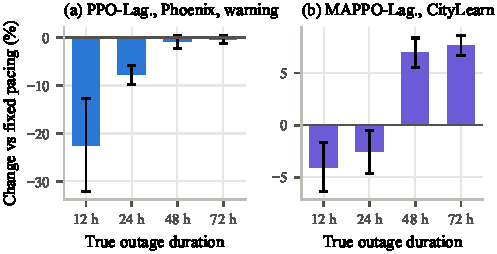
\includegraphics[width=\columnwidth]{fig_learning.pdf}
\caption{Change in vulnerability-weighted degree-hours of the learned policy relative to the fixed-pacing shield on test outages, by true outage length (mean $\pm$ s.d.\ over seeds). Medical losses: zero for PPO-Lagrangian, lower than fixed pacing for MAPPO-Lagrangian.}
\label{fig:learning}
\end{figure}

\begin{table*}[t]
\centering
\caption{Ablations in Phoenix, one change per row. W: 24\,h warning. $\Delta$: first option minus second (negative favours the first). 95\,\% bootstrap interval for $\Delta$VDH; $p$: Wilcoxon signed-rank test on VDH. Paired over the 32 test outages, or $^\ddagger$all 112 outages. $^\dagger$Learned policies averaged over 5 seeds per outage.}
\label{tab:ablations}
\setlength{\tabcolsep}{6pt}
\begin{tabular}{llrrl}
\toprule
Change & W & $\Delta$Dev.-h & $\Delta$VDH [95\,\% CI] & $p$ \\
\midrule
Shield vs.\ weight (greedy) & no & $-$105.0 & 183 [141, 230] & $2\times10^{-9}$ \\
Shield vs.\ none (PPO-Lag.)$^\dagger$ & yes & $-$146.9 & 434 [365, 507] & $5\times10^{-10}$ \\
Health twin vs.\ building order$^\ddagger$ & no & 0.0 & $-$822 [$-$941, $-$708] & $4\times10^{-20}$ \\
Twin vs.\ headcount reward$^\dagger$ & yes & 0.0 & $-$9 [$-$12, $-$5] & $3\times10^{-4}$ \\
PPO-Lag.\ vs.\ fixed pacing$^\dagger$ & yes & 0.0 & $-$153 [$-$185, $-$121] & $5\times10^{-10}$ \\
Warning vs.\ none (shield) & -- & 0.0 & $-$944 [$-$1{,}070, $-$809] & $5\times10^{-10}$ \\
Forecast $\tau_{90}$ vs.\ 48\,h$^\ddagger$ & yes & 0.0 & $-$88 [$-$103, $-$75] & $1\times10^{-19}$ \\
Forecast $\tau_{90}$, $\hat\tau$ vs.\ fixed$^\ddagger$ & yes & 0.1 & 278 [208, 349] & $1\times10^{-8}$ \\
\bottomrule
\end{tabular}
\end{table*}


\subsection{Robustness}
Table~\ref{tab:robust} repeats single-outage sensitivity tests over all 28 start days. Under every perturbation the shield lost at most 0.9 device-hours per 48\,h outage (1.8 at 72\,h), against 116--171 (232--287) for weighted priority. Medical losses rose only with a fully optimistic solar forecast ($\alpha=1$), which supports a conservative factor. A $\pm2^\circ$C temperature-sensor bias changed PH$_{32}$ by about 3\% but not medical service. Shrinking the battery from 150 to 100\,kWh raised the weighted controller's losses from 138 to 171 device-hours, while the shield stayed at 0.1.

\begin{table}[t]
\centering
\caption{Robustness, 48\,h outages, mean over 28 start days, one factor varied at a time.}
\label{tab:robust}
\setlength{\tabcolsep}{3pt}
\begin{tabular}{llrrrr}
\toprule
 & & \multicolumn{2}{c}{Device-h} & \multicolumn{2}{c}{PH$_{32}$} \\
\cmidrule(lr){3-4}\cmidrule(lr){5-6}
Factor & Level & Weight & Shield & Weight & Shield \\
\midrule
PV forecast factor $\alpha$ & 0.4 & 138.4 & 0.0 & 521 & 534 \\
PV forecast factor $\alpha$ & 0.7 & 138.4 & 0.1 & 521 & 536 \\
PV forecast factor $\alpha$ & 1 & 138.4 & 0.9 & 521 & 537 \\
Sensor bias ($^\circ$C) & $-$2 & 116.1 & 0.1 & 548 & 548 \\
Sensor bias ($^\circ$C) & 0 & 138.4 & 0.1 & 521 & 536 \\
Sensor bias ($^\circ$C) & +2 & 155.7 & 0.1 & 494 & 519 \\
Battery (kWh) & 100 & 170.5 & 0.1 & 522 & 542 \\
Battery (kWh) & 125 & 154.8 & 0.1 & 521 & 539 \\
Battery (kWh) & 150 & 138.4 & 0.1 & 521 & 536 \\
\bottomrule
\end{tabular}
\end{table}


\subsection{Price of the guarantee and value of a warning}
The reserve costs comfort. In Phoenix, PDH rose by 3.4\% under the shield (4,073 to 4,211), which is 16.5\% above the perfect-foresight bound (3,613). The unshielded MPC reaches 3,727 by spending energy the shield keeps for medical devices. Because the thermal floor sets cooling for every shielded policy, the shielded MPC coincided with the greedy shield on heat; only the release rate and the sharing of extra cooling are left to the wrapped policy, which is why we learn those. In CityLearn, where each home holds its own 13.5\,kWh battery, the price was larger: 25\% more PDH and 44 against 32 person-hours above 32.2$^\circ$C. A 24\,h warning lowered heat exposure for every controller, by 13\% VDH for the fixed-pacing shield and 15\% for PPO-Lagrangian, and in CityLearn it reduced the shield's losses from 6.1 to 4.1 device-hours.

\section{Discussion and Limitations}
Weighted priority failed in three ways: in the within-hour ranking, when a hot home outranks an oxygen concentrator; in spending energy over time under an uncertain restoration time; and through sensitivity to tuning that differed between platforms. A constraint enforced at run time removes all three regardless of the policy inside it, which is what makes it safe to place a learned policy there. The shield guarantees floors rather than ranking people, which makes it easier to contest and audit. A system making health-relevant energy decisions would likely be classed as high-risk AI in critical infrastructure.

The learning results are modest and depend on context. Learning helped only where the shield left a decision open, after a warning in Phoenix, and both learned policies gained mainly on short outages, because without the true duration they cannot know when early release pays off. Two findings point to the forecaster as the next lever: recorded Arizona outages are far shorter than the 48\,h assumption, and a calibrated duration estimate could become an input to the policy. Pacing to the forecast median, however, was harmful against long outages.

Medical protection and thermal safety compete for the same energy. In the hottest outages indoor temperatures still exceeded $32.2^\circ$C under every controller, including the perfect-foresight bound, so no allocation rule alone can keep residents safe without more storage or cooling-efficient buildings. These results come from simulation. Residents and health-twin weights are synthetic; each platform covers one city and one month at an hourly step; neither includes distribution-network constraints; and the Phoenix building model is calibrated on energy use, not measured indoor temperatures. CityLearn's LSTMs were trained with working cooling and may be unreliable when cooling is shed for long periods, so we emphasise PH$_{32}$, which is less sensitive to extreme values. The CityLearn results rely on the islanding workaround described above and use the base shield. The learned policies were trained on one month of one climate, and MAPPO for only 320 outages. EAGLE-I measures county-level events, which approximate but do not equal the outage seen by one home, and the perfect-foresight bound minimises unweighted rather than vulnerability-weighted heat.

\section{Conclusion}
Treating older adults' medical equipment as a hard, shielded constraint rather than a weighted objective nearly eliminated medical-device outages on two platforms driven by measured data, and remained robust to forecast error, sensor bias and battery size. Ordering the thermal floor by a health twin cut vulnerability-weighted heat exposure by 11\% at no cost to medical service. Learned policies inside the shield stayed safe: PPO-Lagrangian improved on fixed pacing when a warning left energy to allocate, and MAPPO-Lagrangian traded some heat exposure for fewer medical losses. A forecaster trained on a decade of public outage records gave calibrated worst-case restoration times. Next steps are to give the learned policies the forecast as an input, to train MAPPO longer on larger communities, to inform the health twin with clinical and wearable data, and to validate the approach with metered data from homes and care facilities.

\section*{Data and Code Availability}
Weather (ERA5 via Open-Meteo), building loads (NREL ResStock), CityLearn and EAGLE-I are public. One script regenerates every result, table and figure in this paper from these inputs. [Repository link to be added.]

\section*{Author Contributions}
K.~N., A.~Prasad and P.~M.~Ganesh contributed equally to this work. P.~Madhavan supervised the work. % Authors: replace with your agreed contribution statement (e.g., CRediT roles).

\section*{Acknowledgment}
This work received no external funding. Simulations and training were run on the authors' personal computers. Weather data were generated using Copernicus Climate Change Service information (ERA5), accessed through Open-Meteo; outage records are from the EAGLE-I dataset of Oak Ridge National Laboratory, and building loads from NREL ResStock. The authors used Claude (Anthropic) to help write and debug code and to prepare an early draft of the manuscript. The authors revised the text, verified all code and results, and take full responsibility for the content of this paper.

\bibliographystyle{IEEEtran}
\bibliography{refs}

\end{document}
